\begin{savequote}[8cm]

  We hear a lot these days about genes and molecules, but how does one human brain, or one human being coordinate, or entrain, or resonate with another?  We may not realise it, but we live in a world of coordination, at every level and every scale of endeavour.

\qauthor{--- J. A. S. Kelso  \textit{Coordination and the Complimentary Nature} Presentation to the New York Academy of Sciences - May 12, 2010}

\end{savequote}



%It takes two to know one.

%\qauthor{--- Gregory Bateson}


\chapter{\label{chap:theory}A general account of team click in group exercise}

\minitoc


                                  \begin{CJK}{UTF8}{gbsn}

\section{The development of visceral agency in rugby's newest recruit\label{sect:SHW}}
Sun Hongwei arrived, escorted by his high school athletics coach, to the Beijing Temple of the God of Agriculture Sports Technology Institute (\textit{Beijingshi xiannongtan tiyujishu yundong xuexiao} 北京市先农坛体育技术运动学校,
hereafter the Institute) soon after I began my fieldwork in August 2015.  An 18-year-old with a slight build and timid demeanour---his gaze remained diverted to the ground during his first few months at the Institute---Hongwei later told me that he had never seen a rugby ball before that day he arrived.

Hongwei was from Hebei province, immediately surrounding the special prefecture of Beijing, China's capital.  Hongwei's coach had organised a trial for Hongwei with the Beijing Provincial men's and women's Rugby Program (hereafter the Program) by calling upon social connections to the leadership of the Institute.  Athletes come to the Rugby Program from all over the country.  As I explain in more detail in Chapter~\ref{chap:researchSetting}, to represent Beijing at a provincial level in a sport like rugby can translate into the opportunity to gain entrance to one of China's top universities and enhanced career employment opportunities thereafter.

Rugby is not a popular sport in China, but its recent inclusion in the Olympic games (in the form of the modified seven-a-side version of ``rugby sevens'') means that it now occupies a prominent place in the Chinese sport system.  Rugby programs such as the one at the Institute now exist in 12 of China's 34 provincial level regions, either embedded within, or somehow associated with, tertiary education institutions.  Thus, although rugby and China are not commonly associated terms, rugby now affords Chinese athletes a rare and under-capitalised opportunity to pursue attractive life-course opportunities of education and employment in an intensely competitive education system.

Without exception, the athletes who arrive at the Institute to join the rugby team are not like me. They have not spent their childhoods playing rugby in their schoolyards or watching professional rugby on television. Many who come to rugby transition from other more popular sports such as athletics, basketball, or association football, and often---like Hongwei---have never seen a rugby ball before they arrive.  Most athletes start from scratch, so to speak, in terms of their grasp of the requirements of the highly interactive and technically complex team sport.  In addition to complex patterns of movement coordination, rugby also involves unrestrained body-on-body collisions and intense bouts of high physiological exertion.  To perform all of rugby's technical requirements successfully requires a combination of speed, strength, agility, and endurance (see Chapter~\ref{sect:rugbyUnion}).  Learning the game of rugby from a baseline of essentially zero, while also navigating the inevitably demanding social and political dynamics within the team and the Institute, was clearly going to be a daunting task for Hongwei.


                        \begin{center}
                            * * *
                        \end{center}

Even compared to other newly arrived junior athletes, I noticed that Hongwei was particularly timid and shy, especially in his interactions with the senior players and coaches (myself included).  Nevertheless, Hongwei clearly signalled diligence and commitment through his participation in team activities.  He arrived early to each training session, and carried more than his fair share of the training equipment---a task shared by the most junior members of the team.  Each time I passed Hongwei in the corridors of the Institute, he would greet me with a polite bow and greeting: ``Hello, Coach'' (\textit{'jiaolian hao'} 教练好).  In these instances, Hongwei would coordinate his greeting with a moment's eye contact, only to return his gaze to the floor and continue walking.

Due to his lack of familiarity with the basic techniques of rugby, Hongwei was initially unable to fully participate in normal training with the rest of the team.  Instead, during the first month or so, Hongwei remained on the sidelines of the field and practised the basics with other athletes who were unable to fully participate in training due to injury. He began with the absolute basics: learning how to pass and catch the rugby ball, while stationary and while running in-motion. In my eyes at least---eyes of an observer accustomed to instinctual grasp of these movements from a young age---I found Hongwei's attempts to accustom himself to the skills of rugby jarring. The idiosyncrasies of rugby's ovular ball often foiled him.  I would regularly see him on the sidelines of training chasing after a ball that he had just fumbled; the idiosyncratic shape of the ovular rugby ball meant that it would change direction like it were a scurrying rabbit tactfully evading its pursuer.

                            \begin{center}
                                * * *
                            \end{center}

I interviewed Hongwei approximately six weeks after he arrived at the Institute.  Hongwei's demeanour during the interview was consistent with the timid and shy one that he presented publicly at training.  As I explain below, he did show some signs of captivation with his new sport and social environment.  When I asked about his initial impressions of the on-field demands of rugby, however, Hongwei was quick to confess that he felt utterly unacquainted:

  \begin{quote}
    SHW: I still haven't really started to practise any of the team plays or anything; all I can do so far is pass and run a little bit...(but) it's quite fun! \\
    JT: What do you think is the most difficult component of rugby? \\
    SHW: Um\textellipsis well, coordinating with teammates [on the field], particularly coordination in attack.  Because I can't figure it out.  When I first arrived, I didn't even know what a ``switch play'' or a ``blocker play'' was.
  \end{quote}

  \begin{quote}
    SHW: 战术没怎么接触,就是像传球啊、跑动什么的会一点了 \\
    JT: 感觉怎么样?\\
    SHW: 挺好玩的!\\
    JT: 你认为橄榄球最难的一部分是什么? \\
    SHW: ...打配合,进攻的配合,因为搞不明白,刚来的时候也不知道什么交叉,后插什么的 \\
  \end{quote}

Hongwei was self-critical in this confession regarding his minimal grasp of the technical requirements of joint action in rugby.  The obvious stress and anxiety he expressed was indicative of a broader trend with the other athletes I interviewed, as I will explain in more detail in the ethnographic sections of this thesis (see Chapters ~\ref{chap:ethnoField}\nobreakdash~\ref{chap:ethnoResults}). When athletes were asked in interviews about the most difficult aspect of rugby, on-field coordination with teammates was by far the most common answer, particularly among the new recruits and most junior athletes.

As I directed the interview towards topics beyond the on-field technical demands of rugby, Hongwei was more positive, framing rugby as an exciting new opportunity, and commenting that his friends and family were in awe of the fact that he is playing such an impressively ``strong'' (\textit{qiangzhuang} 区壮) physical sport like rugby.  When I asked him about something new that he had learnt through playing rugby, Hongwei automatically responded by emphasising the social dimensions to his experience at the Institute:

  \begin{quote}
    ...I think it's mainly this thing of having teammates. Before, when I was training for an individual sport, it was just me training by myself. [In that environment] it was a case of whoever trained well was successful.  But now with this team of brothers, elder teammates will take care of younger teammates. We all train together, and if you can't do something, you can always ask your elder teammates...[Rugby] is so much better, because in an individual sport, if you can't master something, you have to go to your coach for help. Other athletes don't want to teach you, because if you surpass them, then they have to work even harder to keep up... I have had to learn about helping others, because rugby is not like an individual sport, where you look after your own performance and that's it.  In a team sport, if you don't do well, there's no need to get too frustrated or upset, because other athletes will help you out, and I will also help others out---that type of collaboration with each other.
  \end{quote}

\begin{CJK}{UTF8}{gbsn}
  \begin{quote}
    我觉得主要是师哥师弟的这一块儿,原来练个体项目都是自己练自己的,谁练好了谁厉害,但是现在师哥师弟,有师哥照顾师弟带着,互相练,我不会我可以问师哥
    ...因为个人项目你不会就必须要找教练,但是别人不愿意教你,因为你把别人超越了那别人还还得努力。 学到互相帮助,因为向个体项目自己成绩自己来拿就行,而像团体项目,即使自己做不好,也不用太泄气太沮丧,因为别人会帮你做好,我也会帮别人做好,互相协作的那种.
  \end{quote}
\end{CJK}

Hongwei's explicit reference to the collegiality of the team, and his position as junior member, highlights that the technical skills of rugby were not the only novel components of his experience.  Hongwei's background was in athletics (his event was pentathlon, very much an individual sport), and the team environment was completely new to him.  This was also the case for many of the other athletes in the team.  As I listened to his reflections about rugby and group membership, I could not help but associate the quality of these explicit declarations of group membership with his overly mechanical imitation of rugby's foundational techniques.  In both, I saw his willingness and desire to signal commitment; but both lacked---at the outset at least---a certain level of grasp or conviction.  In the case of his explicit celebration of rugby's social resources in interview, for example, I got the impression that Hongwei was telling me what he thought he ought to say, without deeply believing these things to be unequivocally true.


                            \begin{center}
                                * * *
                            \end{center}

A few months passed, and Hongwei continued to train.  He was as eager and committed as when he began, and I did notice some gradual improvement in his grasp of rugby's basic skills.  But he also remained extremely reserved, keeping his head low at all times in team settings, unless addressed by senior players or coaches.

Then, one evening when I had returned to my room in the Institute dormitory from a three week hiatus in Australia for Christmas, I heard a knock on my open door, and to my surprise Hongwei took an assertive stride into my room, carrying in two arms a draw-string bag containing rugby balls (which were in need of more air before the next day's training session).  Hongwei had never ventured into my room before, apart from when I invited him in for our first interview two months earlier---but certainly never before had he entered on his own accord.  Hongwei looked me straight in the eyes with his head held high and energy radiating from his face and upright chest.  I could not help but smile and ask, with genuine intrigue, ``How have you found training recently?'' (最近练得怎样?)
``Very good'' (很好)he said, assertively and excitedly.  ``Much better than before.  At least now I know what's going on at training, I can keep up with the plays!'' (比以前好多了, 至少现在训练的时候知道该干什么,战术什么的能跟得上!) A big smile spontaneously grew on his face as he continued to hold my gaze confidently.  ``Oh good!'' I said, a little bit shocked.  I congratulated him for his hard work in training while I had been away, and encouraged him to keep at it.  At this, Hongwei took leave by bowing politely and saying ``Thanks, Coach'' (谢谢教练).  ``Wow,'' I remember thinking to myself.  What quantity had all of a sudden possessed Hongwei? Was it possible that his diligent adherence to rugby over those first four months at the Institute had instilled him with a visceral sense of personal and social agency?

                          \begin{center}
                              * * *
                          \end{center}











\section{A general account of team click in group exercise}

How can we scientifically account for the unmistakably visceral and agentic quality of Hongwei's transformation from timid newcomer to budding Beijing rugby player?  As the story of Hongwei anecdotally suggests, the physical and social dimensions of experience in group exercise may take time to develop.  Presumably in Adrian I witnessed the finished product: through many years of on- and off-field engagement with the sport of rugby, Adrian came to personally embody rugby as a social identity, and was thus able to profess its carnal mystery from a place of deep, intuitive knowing (see Chapter~\ref{sect:adrian}).  When I met him during my first stint of research at the Institute, Hongwei was only just beginning this journey.  Over an extended period of ethnographic research it became clear to me that---for Hongwei and others like him---a combination of an increase in familiarity with the on-field technical requirements of rugby and increased familiarity with the off-field social regularities of being an athlete at the Institute brought an increase in personal confidence, and a sense of group membership.  As explained in the previous chapter, a scientific theory capable of accounting for these dynamic and interlocking physical and social dimensions of group exercise is yet to be fully formulated.

In this chapter, I draw on existing empirical evidence and prevailing dynamical theories of social cognition to formulate a novel theoretical account of team click in group exercise.  I introduce the phenomenon of team click as a psychological construct capable of explaining the relationship between joint action and social bonding in group exercise settings.

I begin by reviewing empirical evidence for the phenomenon of team click, noting team click's visceral and socially agentic experiential dimensions.  Following this empirical grounding of team click, I then develop a novel theory of team click in group exercise.  This theory is based on a dynamical conception of joint action, in which physical and social processes are integrated into one overarching inferential framework driven by the mandate of reducing uncertainty.
  Drawing upon this relationship, I hypothesise that the visceral and socially agentic dimensions of team click arise from more positive perceptions of team performance, and, in turn, lay the foundation for processes of social bonding. In addition, I propose that positive violations of team performance may function as an important precedent to team click, directing attention to its visceral and socially agentic dimensions.

Following this theoretical review, I outline the research hypotheses of a general account of team click in group exercise, which I subsequently test via ethnographic and field experimental research.

%First application of AIF to real-world multi-agent joint action scenario (group exercise).


%The theory proposed herein builds upon the hypothesis that group exercise is causally relevant to processes of social cohesion \citep{Dunbar2010,Whitehouse2014,Cohen2017}.
%Synchrony and mimicry literatures:
%The link between joint action and social bonding is well established in the behavioural mimicry and symmetry literatures \citep{Chartrand2009,Launay2016,Mogan2017}, but these studies do not investigate variation in uncertainty of joint action or evaluations of performance as a predictor of social effects.

%UNCERTAINTY

%of JA (suggested in the introduction), or its visceral and social dimensions (SHW as example, Adrian).The role of cognitive uncertainty and unpredictability in dynamical and complex joint action scenarios on processes related to social bonding has not yet been the subject of focussed empirical research.The physical--social link in joint action can be understood as a functional solution to the inherent uncertainty of joint actionPhysical and social represent two ends of a continuum of cognitive strategies deployed by humans to reduce uncertainty inherent in joint action scenarios.The result of effective physical coordination is enhanced social communication (including affective processes of affiliation and connection).  Likewise, effective social communication serves to establish, sustain, and enhance coordination of physical movement in joint action.

%As I explain in more detail below, there is evidence to suggest that the combination of cognitive complexity and physiological exertion in group exercise contexts will necessitate the deployment of more dynamical mechanisms of movement regulation in order to successfully establish and sustain joint action.  In turn

%team click
%The phenomenology of team click captures a scenario in which coordination in joint action is perceived to be either optimal or maximal.  The visceral, and agentic dimensions of team click appear to set the foundation for high quality social bonding among co-actors.  While the social relevance of team click and the related concept of flow have evaded rigorous analysis within more traditional paradigms of social cognition \citep[for explanations as to why, see][]{Dietrich2004,Slingerland2014}, within the novel theory of social bonding through joint action proposed herein, team click can be explained in naturalistic terms as a special case of joint action in which the bonding effects of movement coordination are maximised.


\section{The empirical phenomenon of team click \label{sect:teamClickEmpirical}}
In this section, I draw upon evidence from sporting anecdote, psychology, and anthropology in order to outline the empirical foundations for the phenomenon of team click.  In addition, I point to evidence for team click as an explanatory construct linking joint action and social bonding in group exercise---a proposal which I justify theoretically in the following section.

One of the big mysteries of competitive team sport, particularly at the elite level, is the elusiveness of peak team performance.  While each individual athlete may exhibit expert-level competence in sport-specific skills, the much sought after aggregation of these components, i.e., a team that consistently performs ``in the zone,'' and ``firing on all cylinders,'' in reality often proves frustratingly difficult to achieve and sustain.  As \textcite[568]{King2011} note in their ethnography of the 2008 Cambridge University rowing crew who participated (and who were eventually victorious) in the famous annual Boat Race against Oxford University, the search for collective rhythm is a universal in human social interaction, but  the physiological and psychological complexity of finding that rhythm ``...is extremely difficult to attain; collective performance is a possibility not a certainty.''   The moment in which everything ``clicks'' into place in team sport can, for various reasons, disappear as abruptly as it arrives, if indeed it arrives at all.

When team click is somehow cultivated, and even sustained, it is celebrated as the ultimate, albeit often inexplicable magic of sporting feats. Consider Leicester City Football Club's unbelievable outhouse-to-penthouse title run in the 2015 English Premier League, the recent dominance of the Golden State Warriors in the American National Basketball Association (NBA), or the astonishingly consistent performance of the New Zealand men's national rugby union team (the ``All Blacks'').\footnote{The All Blacks are arguably the most successful sporting team ever, with a winning percentage of 77\% in the last 150 years (and 88\% in the last 6 years) \citep{Kerr2013}.} All of these successful teams carry with them a powerful ``aura'' associated with their capacity to effectively coordinate their behaviours on the field over extended time scales: individual games, seasons, and, in the case of the All Blacks, entire generations.  The aura associated with such rare instances of sustained collective performance in elite sport can spur limitless fascination, fandom, and elaborate exegesis.

    %In this thesis I commit to the more banal task of naturalising the phenomenon of team click, by locating it within a novel theory of social bonding through joint action.

For athletes, coaches, and spectators alike, team click can be a hugely powerful sensation.  As theologian Michael Novak explains, ``[f]or those who have participated on a team that has known the click of communality, the experience is unforgettable, like that of having attained, for a while at least, a higher level of existence'' \citep[11]{White2011}. For the purposes of this thesis, I use the term team click to describe the phenomenology or perception of peak performance within a team of athletes engaged in joint action, but the term has potentially broader applications beyond group exercise (for example, in music making, spoken conversation, or other similar activities).

As explained in Chapter~\ref{sect:linksComplexClick}, the experience of optimal performance in sport has been extensively documented in the psychological literature of flow \citep{Csikszentmihalyi1992,Jackson1995,Jackson1999,McNeill1995}.  Psychologists and neuroscientists have scientifically studied the experience of flow, and have tabled a series of neuropharmacological \citep{Boecker2008}, neurocognitive \citep{Dietrich2006,Dietrich2011,Labelle2013}, and psychological \citep{Csikszentmihalyi1992} theories for its emergence.  The vast majority of flow research has focussed on the experience of the individual---the athlete, musician, or performer.  Some attempts have been made to extend an analysis of flow and its antecedents to the level of the group and dynamics of interpersonal coordination---a phenomenon termed ``group flow'' \citep{Sawyer2006}---but these attempts lack coherence and development.  Anecdotal and observational evidence suggests that in addition to the components of flow already identified at the level of the individual, successful performance of technically complex
\textit{joint} action could have distinct psychological and social consequences.

In this thesis, I suggest that team click is distinct from flow in that it specifically delineates perceptions of joint action from individual action, and therefore implicates physiological, cognitive, and social mechanisms unique to joint action \citep{Vesper2010}.  In particular, team click in joint action entails an added level of complexity owing to the cognitive uncertainty inherent in coordinating behaviour with autonomous co-actors.  As I explain in more detail in the theoretical section below, there is evidence to suggest that the cognitive uncertainty of dynamic joint action may also be the source of social effects characteristic of social bonding, specifically when the uncertainty of joint action is mitigated via successful coordination of movement.


\subsection{Phenomenological components of team click}
It is reasonable to assume that the psychological phenomenon of team click will share many similarities with the visceral and autotelic components of experience associated with flow \citep{Sawyer2006}.  In addition, it is likely that team click will involve an extra phenomenological dimension, owing to its inherently social features.  Team click is anecdotally present in a wide range of joint action contexts, and is often associated in these contexts with psychological processes of positive affect and wellbeing, as well as personal and social agency, social affiliation, and group membership \citep{Jackson1995,Marsh2009,Wheatley2012,Slingerland2014}.

Tightly synchronised activity in particular, found in team sports such as rowing, can help dissolve the boundaries between individual and social agency: ``In rowing...it feels like you have at your command the power of everybody else in the boat. You are exponentially magnified. What was a strain before becomes easier. It is absolutely the ultimate team sport'' \citep[x]{Brown2016}.
The blurring of agency between self and team may be responsible for facilitating affiliation and trust between teammates in competitive athletic environments such as professional rugby, which often involves high physiological stress and uncertainty.  As Jeremy Paul, a famous Australian Rugby player commented of his late teammate, Dan Vickerman:

      \begin{quote}
        ...you always wanted a guy who would go into the trenches with you and he always played consistently well...he could really play and was just one of the good lads that you enjoyed his company \citep{Fox-Sports2017}.
      \end{quote}

As this excerpt suggests, the experience of team click may act as a social diagnostic tool, whereby perceptions of successful performance with co-actors could drive attribution of social inferences of competence and reliability to co-actors.

The experience of team click, like flow, also often involves an experience of awe or exhilaration arising from perceptions of successful performance of joint action.  While elite athletes presumably always aim for optimal performance in joint action, the experience of achieving that desired state, and even exceeding it---often with the help of co-actors---appears to be a powerful, and somewhat ``surprising'' experience.  In the 1990s, psychologist Susan Jackson conducted a number of qualitative studies documenting athletes' (in this case elite figure skaters) experience of flow in solo and joint action:

    \begin{quote}
      Oh, it's awesome! Everything's at peace...the crowd was involved, we were involved as a pair team, and we were just aware of everything, it just kept snowballing, like we weren't going to miss, and it was great, it was an awesome experience \citep[168]{Jackson1992}.
    \end{quote}

Here, the athlete appears to be surprised and in awe of the achievement of optimal collective performance.  Part of the awesomeness may derive from the rare feeling of absolute alignment between self and co-actor(s):

    \begin{quote}
      What was really so special about this performance was that there was nothing between (partner's name) and I but flow.  You know, through the whole three minutes.  That meant that her mind and my mind were clear and in the same...in a partnership. It's always adjustments for ``Am I?'' and ``Are You?'' and ``Where Are We?'' and stuff like that.  That day was really a marriage of (partner) and (self) and the ice.  So I think it's a different kind of flow experience than a single skater who has much more control over themselves. \citep[173-4]{Jackson1992}.
    \end{quote}

This passage draws attention to the fact that joint action---more so than individual action---entails additional cognitive demands of attending to the movements and intentions of others \citep{Vesper2010}.  The achievement of click in joint action appears to be associated with the reduction or down-regulation of cognitively effortful processes of monitoring self and other contributions to joint action \citep{Dietrich2004b}. Research suggests that optimal coordination in joint action may be defined by a combination of patterns of fluent, ``co-confident'' movement \citep[in place of effortful monitoring; see]{Noy2015,Noy2017}, and a ``we-mode'' of social agency in which the contributions of ``you'' and ``I'' are momentarily transcended or abandoned \citep[see][]{Gallotti2013}.
The experience of team click could therefore be a powerful signal of shared commitment to joint action and willingness to cooperate \citep{Reddish2013a}. \\

In sum, team click refers to perceptions and experiences of peak team performance in group exercise contexts.  Based on this brief review of anecdote and evidence from psychology, anthropology, and further afield, an individual's perception of team click should contain some or all of the components outlined in Table ~\ref{tab:teamClickComponents}.  Team click can involve perceptions of tacit (rather than explicit) understanding between co-actors, experience of autotelic flow or coherence of joint action, a quality of aura or atmosphere around the team, a blurring of agency between self and teammates or group, and perception of reliability of others and self in performing their roles.  These six phenomenological components of team click can be reduced to two main dimensions: viscerality, and social agency.  As I develop in more detail in the theoretical section of this chapter, there is evidence to suggest that the combination of viscerality and social agency provide a cognitive template for processes of social affiliation and identification characteristic of social bonding.

% Please add the following required packages to your document preamble:
% \usepackage{booktabs}
\begin{table}[]
  \centering

\begin{tabular}{@{}ll@{}}
\toprule
\textbf{Component} & \textbf{Description} \\ \midrule
 &  \\
\textbf{Viscerality} &  \\
 &  \\
Tacit understanding & \begin{tabular}[c]{@{}l@{}}Perception of unspoken or implicit alignment\\ of expectations with co-actors\end{tabular} \\
 &  \\
Group flow & Perception of flow or coherence in joint action \\
 &  \\
Atmosphere or aura & \begin{tabular}[c]{@{}l@{}}Perceived positive, energetic quality within \\ or surrounding the team\end{tabular} \\
 &  \\
 &  \\
\textbf{Social Agency} &  \\
 &  \\
\begin{tabular}[c]{@{}l@{}}Blurring of self \\ and other agency\end{tabular} & \begin{tabular}[c]{@{}l@{}}Blurring of distinction between self and other\\  agency in joint action\end{tabular} \\
 &  \\
\begin{tabular}[c]{@{}l@{}}Ability extended \\ by others\end{tabular} & \begin{tabular}[c]{@{}l@{}}Feeling that individual abilities are extended\\ by the agency of others\end{tabular} \\
 &  \\
\begin{tabular}[c]{@{}l@{}}Reliability of self\\  and others\end{tabular} & \begin{tabular}[c]{@{}l@{}}Perceived certainty concerning the ability of \\ self and others to contribute effectively to joint action\end{tabular} \\
 &  \\ \bottomrule
\end{tabular}

\caption{Phenomenological components of team click}
\label{tab:teamClickComponents}
\end{table}



\subsection{The theoretical challenge for a scientific understanding of team click}
Researchers have pointed out that flow---a concept that shares many similarities with team click---has traditionally escaped rigorous scientific analysis \citep{Dietrich2010a,Slingerland2014}.  Dietrich, for example, explains that flow presents a paradox that is difficult to explain according to traditional theories of attention and mental effort, which tend to assume that better performance, on any task, is associated with increased conscious effort allocated to that task \citep{Dietrich2004b}.  As \textcite{Slingerland2014} surmises, flow reflects a paradox in which an individual in flow appears to be ``trying not to try.''  Flow appears to entail spectrum of both effortful (intentional, mental) and seemingly effortless (implicit, automatic) cognitions---some of which appear to depend on the resources beyond the brain.  Team click, like flow, is a multidimensional process involving mental, embodied, emotional, and social dimensions.  In this thesis, I consider the suggestion that the most effective way to reconcile the analytical paradox associated with flow, team click, and the mystery of group exercise more generally is via a more dynamical and integrative model of cognition \citep{Clark2015}  In the sections that follow, I outline the building blocks necessary to formulate a novel theory of social bonding through joint action.


%This passage demonstrates the key elements of distinction between the experience of click in solo and joint action. As I will explain in more detail below, joint action requires constant finessing (adjustments) of behaviours and intentions between co-participants in which individuals are consulting internal models of self, other, and joint action \citep{Pesquita2017}.


%a direct link between dynamical coordination of physical movement and social communication, and


\section{A theoretical account of team click in group exercise}

To formulate a general account of team click in group exercise, I begin by developing a theoretical grounding for team click based on the proposed relationship between uncertainty and coordination of physical movement and social communication in joint action.  Emerging dynamical perspectives on social cognition suggest that positive perceptions of team performance in joint action and social bonding may be causally linked by an overarching mandate to reduce levels of uncertainty in joint action.  I suggest that the visceral and socially agentic experiences of team click can be explained as responses to instances of \textit{unexpected} success in team performance.  In particular, positive violation of expectations concerning team performance could set the foundation for experiences of social agency and viscerality.  Finally, I present evidence to suggest that experiences of agency and viscerality characteristic of team click could serve as a necessary sensorimotor foundation for more elaborate and culturally-mediated processes characteristic of social bonding.  In fact, as I explain below, a dynamical theoretical approach to social bonding suggests the reverse: social heuristics, rationalisations, beliefs, and group identities characteristic of social bonding serve as functional affordances through which brains reduce the ``mystery'' of social interaction.  Together, these components form a general theoretical account of team click in group exercise, whereby team click mediates a relationship between perceptions of team performance and social bonding.

Following this review, I formulate two hypotheses.  The first hypothesis proposes a relationship between perceptions of team performance and social bonding, mediated by team click (H1).  The second hypothesis claims that better-than-expected execution of joint action will mediate a relationship between prior levels of uncertainty and team click (H2).  Specifically, higher levels of uncertainty in joint action will lead to higher levels of team click when team performance is perceived to be more successful relative to prior expectations.


%positive expectation violation as an underlying mechanism linking uncertainty in joint action, evaluations of team performance, and team click (Hypothesis 2).



\subsection{Uncertainty and coordination in joint action}
In this section, I outline evidence that substantiates a dynamical relationship between levels of uncertainty and levels of coordination---of physical movement and social communication---as functionally integrated strategies for coping with the uncertainty of joint action.  This physical--social link serves as a foundation for a theory of social bonding through joint action in group exercise.

Emerging perspectives on social cognition suggest that positive perceptions of team performance in joint action and social bonding may be causally linked by an overarching mandate to reduce levels of uncertainty in joint action \citep{Marsh2009,Friston2015a,Pesquita2017}.  Humans are hyper-social \citep{Tomasello2012a}, to the extent that our capacities for social interaction---particularly those that are more basal and implicit, like physical movement coordination---have stabilised as an often taken-for-granted aspect of our phenotypic repertoire \citep{Wheatley2016}.  It is important to realise, however, that successful coordination in joint action poses a cognitively improbable challenge owing to its inherent uncertainty.  It appears that humans deploy a suite of canny physiological and social mechanisms in order to mitigate uncertainty in social interaction.

\myparagraph{Uncertainty}
In this thesis, I define uncertainty as a quantity that reduces an an actor's ability to successfully predict, monitor, and sustain joint action.  Existing evidence suggests that uncertainty---defined in this way---can impact on cognitive processes of decision making. It has also been linked to emotional response and psychopathological disorders.

Most evidence for the effects of uncertainty on cognition comes from decision-making studies.  Decision-making during uncertainty is usually defined as a situation that has limited or incalculable information about the predicted outcomes of behaviour \citep{Huettel2005}.  In general, results suggest that higher levels of uncertainty lead to greater inability to make optimal decisions, particularly when presented with a novel or time-pressured stimulus \citep[versus a stimulus learned through repeated exposures;][]{Daw2005,Kording2006}.  Researchers have also identified the role of executive control on mitigating uncertainty in decision making \citep{Mushtaq2011}, which is bolstered by evidence to suggest  that mitigation of uncertainty via mechanisms of executive control  utilises distinct neural pathways for processing uncertainty \citep{Huettel2005}.  Taken together, this evidence suggests that processes of learning and executive control enhance ability to mitigate uncertainty in decision making.

The effect of uncertainty on physiological and emotional response is less well understood, although results generally suggest that uncertainty is associated with higher levels of stress, anxiety, and autonomic arousal.  Early investigations into the effects of uncertainty on anticipation of pain (electric shocks) showed effects of higher levels of uncertainty on heart rate \citep{Averill1972} and skin conductance \citep{Epstein1970}. More recent studies have shown effects of uncertainty on hormonal \citep[e.g., serum cortisol, see][]{Voigt1990} and immune \citep[e.g., lymphocyte proliferation, see ][]{Zakowski1995} response. These studies showed that prior exposure mitigates the effects of a subsequent manipulation of uncertainty \citep{Voigt1990}, and that predictability buffers the effect of the stressor on immune function \citep{Zakowski1995}.  Uncertainty has been associated with self-reported feelings of stress \citep{Lazarus1985}, threat/challenge \citep{Folkman1985}, and anxiety \citep{Holaway2006}.  Recently, \textcite{Moutoussis2014} reported evidence of higher placebo response to (sham) pain stimulus as a function of higher uncertainty.  While in the case of decision making, uncertainty appears to be mitigated by cognitive control, strategies for physiologically mitigating uncertainty are less clear. Taken together, results suggest that higher levels of uncertainty can impact on cognitive performance, emotional state, and physiological response.
%E: tractability of uncertainty as a variable; need for definition. formal  entropy offers a thermodynamic

With these considerations in mind, I adopt a broad and formal definition of uncertainty which draws upon the notion of Shannon entropy \citep{Shannon1963}.  Shannon entropy itself amounts to a cognitive (information-theoretic) rendering of thermodynamic entropy, which can be understood as a measure of our ability to predict the position of particles within a system over a duration \citep{Linson2018}. Thermodynamic entropy typically increases with heat, since faster particle movement gives off more heat than slower movement, and faster movement leads to more unpredictable positions.  Instead of predicting the location of particles as a function of heat, Shannon entropy concerns predicting the location of a meaningful cognitive signal within varying levels of background noise.  Higher levels of noise lead to higher levels of uncertainty, because the ways in which information can be organised to create meaning increase as the message increases \citep{Shannon1963}. In other words, the greater the ability to predict where the signal is within the noise of all possibilities, the greater the certainty.  Thus, in the sense here defined, higher levels of uncertainty equate to lower ability to make accurate predictions concerning meaningful information contained in the environment.


\myparagraph{Uncertainty in joint action}
Joint action is unique in its uncertainty.  The uncertainty associated with coordinated physical movement in living systems was first described by neurophysiologist Nikolai \textcite{Bernstein1967}.  Bernstein noted that, in the case of human intra-personal movement, an impressive balance is somehow struck between flexibility, precision, and control, whereby hundreds of muscles and joints coordinate to perform many different tasks of everyday life.  When we grasp a cup or catch a ball, many individual muscles and joints---each with their individual degrees of freedom---work together in fine concert.  Bernstein found it unlikely, from a computational perspective, that the central nervous system would be able to finely control all the possible movements (the degrees of freedom) of each single muscle individually to create coherently directed movements---it would be computationally impossible.  Rather, he suggested that muscles and joints form  ``functional synergies''---flexible, function-specific, self-organising assemblies---by locally coupling and constraining each other's degrees of freedom to greatly reduce the amount of control needed.  Thus, Bernstein predicted that successful action control would necessitate dynamical mechanisms of physical movement coordination in concert with executive control functions.

The uncertainty inherent in joint action poses an even greater challenge to successful performance.  Intra-personal and interpersonal human movement both rely on the nervous system's capacity to anticipate, attend, and adapt to the conditions of the environment \citep{Keller2014}.  In the case of intra-personal human movement, successful coordination is made possible by the nervous system's direct access to information concerning the spatiotemporal position of the body and its relationship to the environment.  Privileged access to this information enables habituated coupling of a movement control system to the organism's various degrees of freedom, and therefore the emergence of functional synergies \citep{Riley2011}.  By contrast, interpersonal movement coordination---i.e., joint action---presents an even greater challenge.  In the case of interpersonal coordination, the combination of 1) limited reliability of sensory modalities as a source of information about the action of others \citep{Wilson2005,Wolpert2003,Frith2007} and 2) the informational complexity associated with a cognitive system comprising multiple autonomous agents (each with their own movement degrees of freedom) predicts that successful performance in joint action will be defined by higher levels of uncertainty relative to successful performance of actions under individual control \citep{Turvey1978}.

Cognitive scientist Natalie Sebanz and colleagues \citep{Sebanz2006,Vesper2010} have proposed that joint action requires individuals to adhere to the following minimal conditions:

\begin{enumerate}
  \item Represent a shared goal, as well as representing one's own individual contribution to the shared goal.
  \item Apply monitoring and prediction processes to each partner's actions. This includes monitoring the extent to which shared goals or tasks are being fulfilled while at the same time predicting a partner's actions.
  \item Facilitate continuous coordination via coordination smoothing, defined as the process of continuously improving one's prediction of the partner's action.
\end{enumerate}

Considered from a dynamical perspective, the challenge associated with meeting these minimal requirements will vary as a function of the level of uncertainty in a given joint action scenario \citep{Turvey1982}.  Joint action scenarios subject to experimental analysis usually involve relatively low levels of uncertainty owing to their simplistic structure and task requirements.  The synchrony and social bonding literature, for example, usually involves simple dyadic manipulations of synchrony or joint action, so that variables of interest can be successfully operationalised and manipulated \citep{Launay2016,Mogan2017}.  By contrast, many real-world joint action scenarios are striking for extremely high levels of uncertainty.  Real world joint action scenarios often involve many actors engaged in various hierarchically organised layers of nested joint goals over various spatiotemporal scales that, in turn, recruit various sensory modalities \citep{Keller2014}.  The claim emanating from dynamical social cognition is that solving the degrees of freedom problem in joint action scenarios involving high uncertainty will require sufficiently high levels of coordination---of both physical movement and social communication between co-actors.  As I continue to develop below, this claim sets a theoretical foundation for the phenomenon of team click.

\myparagraph{Uncertainty in group exercise}
Above and beyond normal day-to-day instances of communication and exchange, joint action in group exercise is defined by extremely high levels of uncertainty.  Many group exercise scenarios such as group dancing or sport not only involve complex (i.e., multidimensional) joint action structures (layers, timescales, sensory modalities).  Group exercise contexts also invariably involve ``on-line'' and ``in the moment'' time-pressure demands associated with action selection and executionm, which could place constraints on normal cognitive function \citep[as has been shown in laboratory studies of decision-making studies;][]{Kerstholt1994,Maule2000}.  Moreover, attempts to model and predict the behaviours and intentions of multiple co-actors in joint action scenarios typical of group exercise will entail a high and possibly intractable computational burden, particularly if the number of co-actors in joint action exceeds the known cognitive upper limit for face-to-face interaction of four or five \citep{Dunbar1992}.\footnote{Evolutionary Anthropologist Robin \textcite{Dunbar1992} proposes that the ratio of human neocortex size to total brain volume imposes an upper cognitive limit on real-time coordination of behaviour of approximately four to five individuals.  Many interactional team sports involve five (e.g., basketball) or more (e.g., football, rugby) co-actors.}  In the case of interactional team sports, the presence of \textit{competition} between co-actors \citep[whereby one individual or team of individuals actively attempts to foil or disrupt the actions of another individual or team of individuals;  see][]{Reimer2006} serves to amplify uncertainty in joint action to the extreme.

In addition to these heightened cognitive challenges associated with joint action in group exercise, it has also been suggested that uncertainty in group exercise will be modulated indirectly via the neurocognitive effects of physiological exertion on brain function.  As Neuroscientist Arne Dietrich points out, physical exercise is at its core a stressor that will necessitate an energy trade-off in the brain, whereby energetically costly brain regions inessential to movement execution are temporarily down-regulated \citep{Dietrich2004b}. Neurocognitive down-regulation as a result of physiological exertion could further amplify uncertainty, by reducing individuals' ability to predict and regulate joint action.\footnote{Dietrich suggests that experiences of flow and the ``runner's high'' in exercise could be the result of temporary down-regulation of energetically costly brain regions inessential to movement execution \citep{Dietrich2004b}.  As candidate brain regions, Dietrich and colleagues propose areas of the dorsolateral prefrontal cortex responsible for self-monitoring and proprioceptive sensory attenuation \citep[commonly known as the ``inner critic'' regions of the brain; see][]{Limb2008}.}  Thus, it can be expected that commonly encountered aspects of group exercise---here described mainly in relation to competitive (team) sports---contain high levels of uncertainty, which will constrain usual day-to-day abilities to successfully predict, monitor, and sustain joint action.

As Bernstein pointed out in relation to individual action, it is unlikely that adherence to the minimal requirements of representing, monitoring, and sustaining joint action could be driven solely by central, executive control processes in the central nervous system---joint action would be too slow and costly \citep{Dietrich2004b}.  It is similarly unlikely that processes of unconstrained automatic alignment (with no higher-level coordination) could enable joint action of the type observed in humans \citep{Fusaroli2014}.  Rather, it seems more plausible that joint action is facilitated by a continuum of mechanisms spanning executive control through to more direct physical coupling with the environment \citep{Semin2008,Frith2008}.  Thus, it can be assumed that, based on the sheer uncertainty inherent in joint action (relative to individual action), successful performance will demand a suite of mechanisms---spanning both physical and social domains.

Existing experimental evidence confirms the notion that physical and social processes in joint action belong to a continuum of cognitive strategies that work together to reduce uncertainty.  Humans display fine-tuned sensitivity to the quality of joint action and readily infer social significance from the outcomes of joint action ~\citep{Wheatley2016}.  As early as 1944, psychologists \textcite{Heider1944} demonstrated that complex social intensions and emotions could be deciphered from the motion trajectories of simple shapes, and individuals readily extract social information (such as gender, emotion, and personality) from dynamic point-light displays \citep{Atkinson2004,Johansson1973}.  Neuroscientific evidence suggests that auditory, visual, and biological motion are processed by shared neural cortices \citep[e.g., the right superior temporal cortex; see][]{Zatorre2007,Beaucousin2006,Beauchamp2007}. Patients with aprosodia (inability to convey or interpret dynamical properties of speech) and amusia (the inability produce or interpret music) display correlated deficits in recognising gestures and facial expressions.  Taken together, these findings suggest the existence of shared neural mechanisms for multisensory perception of dynamical motion and social communication \citep{Wheatley2012,Wheatley2016}, which could aid the achievement of minimal requirements of joint action described above \citep{Novembre2014,Sebanz2009}.

%It has been hard to conceptualise the link between the two:CR and MES -- focus on more explicit forms of communication.

In the next section, I introduce core tenets of an emerging paradigm within social cognition that enables the formulation of a novel theory of social bonding in joint action. Foundational to this theory is the way in which higher levels of uncertainty in joint action require higher levels of physical and social coordination in order for joint action to be performed successfully.  As I explain below, there is evidence to suggest that an overarching mandate of uncertainty reduction in joint action necessitates dynamical mechanisms of physical movement coordination, as well as effective and efficient mechanisms of social communication.  As I develop in what remains of this chapter, this dynamical proposal sets the foundation for a relationship between perceptions of success in team performance and social bonding, mediated by the phenomenon of team click.


\subsection{The active inference framework\label{sect:AIF}}
An emerging body of research in cognitive science conceives of physical and social processes associated with action and perception as adhering to an overarching thermodynamic-inspired mandate of reducing uncertainty \citep[referred to as variational or information-theoretic ``free energy''][]{Friston2015}.  Now commonly referred to as the active inference framework \citep[hereafter AIF][]{Friston2006,Friston2010,Clark2015,Linson2018}, this emerging approach enlists the neurocomputational strategy of predictive coding \citep[hereafter PC; see][]{Rao1999} in order to operationalise the concept of uncertainty in the brain as a process of prediction error minimisation \citep{Clark2013}.  PC posits a dynamical and hierarchical process of ``generative modelling,'' in which ``forward models'' for prediction of action and perception are \textit{integrated} into action and perception as the instructions for action and perception themselves \citep[rather than being auxiliary to action and perception;][]{Pickering2014}.  PC allows for the integration of traditionally disparate processes (e.g., physical, emotional, cognitive, or social) in one integrative inferential framework \citep{Clark2015}.  PC thus involves a radical inverse of traditional models of cognition and motor control. Thus far, evidence suggests that PC may offer a more computationally efficient and flexible strategy for brain function and cognitive inference than existing alternatives \citep{Pickering2014,Clark2015a}.  For a more detailed review of PC and the distinction between auxiliary forward models and integrative forward models for motor control, see Appendix~\ref{app2:motorControl}.

In the PC framework, hypotheses concerning likely causes of sensory stimuli are adjudicated by the brain through an inferential process likened to ``empirical Bayes'' \citep{Clark2013}.  Hierarchical predictions are informed by three calculations: 1) prior experience, 2) available sensory evidence, and 3) precision-weighting---a second-order calculation of the relative precision or reliability of the available sensory evidence.  Second-order precision weighting of sensory evidence enables flexible direction of attention to prediction errors occurring at multiple levels of the hierarchical generative model (e.g. lower-order sensorimotor levels or higher-order perceptual or conceptual levels), and deriving from \textit{exteroceptive} (relating to stimuli that are external to an organism, i.e. visual, auditory, haptic perception), \textit{interoceptive} \citep[relating to stimuli produced within an organism, particularly by the body's organs (viscera) e.g., ``gut feelings,'' or elevated heart rate; see][]{Seth2013,FeldmanBarrett2015}, or \textit{proprioceptive} \citep[relating to stimuli that are produced and perceived within an organism, especially those connected with the position and movement of the body; see][]{Friston2011a} information.  Iterative learning adjusts the precision weighting mechanism to strengthen prior probability distributions of models for future inference \citep{Robbins1964}.

In effect, second-order Bayesian inference allows the brain to decide which prediction errors to pay attention to (e.g., exteroceptive, interoceptive, or proprioceptive) at which level of the coding hierarchy \citep[for example, higher conceptual errors or lower sensorimotor errors][]{Friston2015}.  Each error signal is conditioned with a precision weighting, which functions to either ``dial-up'' or ``dial-down'' the volume on that signal's influence on the overall predictive model \citep{Clark2015}.  Precision weightings are proportional to the inverse variance of the model prior for each sensory input \citep{Ernst2004,FitzGerald2014}.  In other words, the volume of more reliable or more commonly encountered sensory inputs will be dialled-up, while the volume on less reliable or less commonly encountered sensory inputs will be dialled-down. This process of precision weighting can be understood as the dynamical social cognition's version of the traditional notion of attention \citep{Ramstead2016}. Bayesian precision-weighting (attention) functions by selectively promoting certain predictions over others as a strategy to reduce overall uncertainty.
Here, the suggested relationship between likelihood and attention also raises the possibility of its inverse, i.e., that less likely events will lead to higher levels of surprise in instances in which unlikely events come to fruition \citep{Chetverikov2016}.  This relationship will be considered at length below in relation to the visceral and socially agentic dimensions of team click.

As a compliment to PC, the AIF also proposes a revitalisation of affordance theory \citep{Gibson1979} in order to theorise the role of extra-neural resources in affording more effective and elaborate strategies in uncertainty minimisation \citep{Friston2012}.  In essence, affordances can be understood as devices to which generative predictive models couple to reduce uncertainty.  Such affordances range in their complexity, from basal affordances of the immediate physical environment, through to cultural affordances, which are coupled to more elaborate and culturally contingent processes \citep{Ramstead2016}.  In the context of joint action in particular, cultural conventions can be understood as shared frames of reference that set the macro-contextual coordinates---or ``hyper-priors'' in PC parlance---for joint action \citep{Clark2013}.

Research suggests that cultural norms function as affordances that smooth coordination via a shared referent for joint action \citep{Vesper2017}. Joint actions that involve complex sequences and divisions of labour between participants appear to rely heavily on capacities to explicitly signal intention for the assigning of roles, forward planning, and repair of failed coordination \citep{Frith2010}.  These ``coordination smoothers'' \citep{Vesper2017} often function to reduce spatial and temporal variation in action by providing a shared spatiotemporal referent for co-alignment of predictions. Taken together, these proposals offer a conceptualisation of the way in which features of a specific activity or cultural context can reliably pattern and shape human experience of joint action, without necessarily altering universally shared cognitive and evolutionary principles of behaviour \citep{Roepstorff2010}. In the ethnographic sections of this thesis, I deploy the concept of cultural affordances (and related terms such as coordination smoothers) in order to render visible the various interacting processes that bear upon athlete experience of joint action in rugby in China (see Chapters~\ref{chap:researchSetting} to~\ref{chap:ethnoResults}).

To summarise, the AIF proposes that physical and social processes in joint action are linked as part of a continuum of strategies that adhere to an overarching mandate of reducing uncertainty.  Traditionally-termed ``lower-order'' cognitive processes of physical movement regulation form the base layer of hierarchically organised predictive models, while traditionally-termed ``higher-order'' cognitive processes associated with executive control and communication form the higher layers of the same model, given that the model successfully serves to reduce uncertainty \citep[over the lifespan of the organism][]{Ramstead2017}.  Thus, in the case of joint action, more successful models will be those which successfully reduce uncertainty through a coordinated assemblages of both physical and social strategies, engaging neural, extra-neural, and cultural affordances \citep{Clark2015}.  The AIF proposes a reconceptualisation of cognition by reconciling traditional boundaries between physical and social processes, through the suggestion of an integrated inferential framework organised in terms of uncertainty minimisation.

%\citep[cf.][]{Kahneman2011}.


%designed---through processes of ontogeny and phylogeny---to reduce uncertainty in humans' thoroughly social evolutionary niche \citep{Ramstead2017}.



\subsubsection{Was it a thief or just the wind?\label{sect:windThief}}
To help develop an intuition for the AIF, in this section I reference a contrived example provided by cognitive scientist Giovanni \textcite{Pezzulo2014}.  (\textit{I will continue to refer to this example throughout this chapter in order to simulate theoretical claims of the AIF}).

Imagine you wake up in the middle of the night to the sound of your bedroom window creaking.  At the higher levels of the predictive coding architecture, competing perceptual hypotheses emerge to explain the likely causes of the sensory experience.  For simplicity, assume that two plausible hypotheses emerge: 1) the wind outside caused the window to creak (wind), or 2) a thief is trying to break in to your house (thief).  The probability that the sensory experience of the window creaking is due to the wind can be represented by the equation in Figure ~\ref{fig:windThief}. The AIF claims that the brain formulates a probability estimate based on:

\begin{enumerate}
\item $P(wind)$: the model \textit{prior} formulated by previous experience (e.g., it has been windy at night recently, or in the case of $P(thief)$, there have been some recent thefts in the neighbourhood)
\item $P(evidence|wind)$: the \textit{likelihood} that the sensory experience is caused by the wind (this value could be informed by other sources of information, e.g., the trees outside are also rustling, the dog is not barking (which may be the case if it were a thief, ($P(evidence|thief)$)
\item Precision weighting: the reliability or certainty associated with your sensory inputs (it is dark in your room and so you may not trust your visual perception, you just woke up so could have been dreaming, etc.).  The precision weight is factored into the ``evidence.''
\end{enumerate}

      \begin{figure}[htbp]
      \begin{center}
      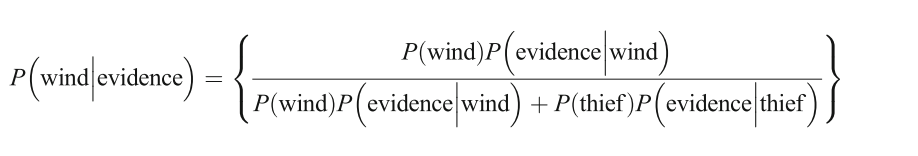
\includegraphics[scale=.5]{images/windThief.png}
        \caption{Bayesian model for the prediction of wind as the cause of the window creaking. Source: Pezzulo (2014)}
          \label{fig:windThief}
      \end{center}
      \end{figure}

These two hypotheses (wind and thief) effectively compete on the basis of how well they explain the sensory stimuli.  The brain's capacity to quantify the uncertainty of any given sensory state facilitates optimal selection between competing predictions pertaining to the same bottom-up sensory signals.  In this example, based on the priors ($P(wind) = .8$ (it has been windy recently) and $P(thief) = .2$ (no recent reports of theft)), and the (precision-weighted) evidence ($P(evidence|wind) = .6$ and $P(evidence|wind) = .5$ (roughly equivalent because it is dark and you have just woken up), the probability of wind ($= .83$) is much higher than the probability of thief ($= .17$).  In this case, the prediction that wind caused the window to creak wins out, and guides action and perception accordingly (e.g., you decide to go back to sleep).

 The ``active'' quality of the AIF refers to its ability to integrate a range of sensory inputs into one overarching inferential process.  Original models of PC dealt primarily with exteroceptive information \citep[relating to stimuli that are external to an organism, i.e. visual, auditory, haptic perception;][]{Rao1999,Friston2010}.  In the wind vs. thief model considered above, for example, only exteroceptive evidence is considered, in the form of the auditory stimulus of the window creaking.  Research has since demonstrated that the PC approach can also account for ``proprioceptive'' information (relating to stimuli that are produced and perceived within an organism, especially those connected with the position and movement of the body), as well as ``interoceptive'' information  \citep[relating to stimuli produced within an organism, particularly by the body's organs (viscera) e.g., ``gut feelings,'' or elevated heart rate; see][]{Seth2013,FeldmanBarrett2015}.  Incorporating proprioceptive and interoceptive information sources into PC allows researchers to theoretically demonstrate that human cognition is both ``embodied''---inference is rooted in and contingent upon visceral, interoceptive information \citep[][]{Pezzulo2014}, as well as ``active''---in the sense that humans can rely on physical movement to reduce the discrepancy between proprioceptive predictions and actual body states, and thereby reduce free energy \citep[see][]{Friston2010,Clark2015}.  In the case of motor systems, agents like humans are able to move their sensors in ways that amount to actively seeking or generating the sensory consequences that they (or rather, their generative models) expect \citep[][1349]{Friston2003}.

To fully comprehend this proposal, consider an active revision of the wind vs. thief example.  Two key differences in the model become apparent.  First, the evidence that the generative model considers is broadened to include both interoceptive and proprioceptive information, in addition to exteroceptive evidence.  Assume that before you went to bed you just watched a horror movie, and when you woke up to the sound of a window creaking, your heart began to pound, and you immediately fixated on the hypothesis that a thief was causing your window to creak.  Immediate fixation on the thief hypothesis can be explained by the contribution of interoceptive information (e.g., autonomic stress response, heart beat, etc.) to the sensory evidence \citep{Pezzulo2014}.  In addition, the incorporation of proprioceptive information into the model (for example, the possibility of moving to turn on the bedside lamp) creates additional cognitive affordances through which higher-level predictions could be strengthened (or uncertainty can be minimised).  This difference in the model demonstrates how perception, emotion, and action are functionally integrated in human cognition under the AIF.

Second, broadening sensory inputs in the model also introduces the problem of differential reliability of sensory inputs.  The wind vs. thief example describes a situation in which exteroceptive information is relatively unreliable: it is dark, so visual inputs are restricted, and what you heard is unreliable because you just woke up, and maybe it was part of a dream.  By contrast, interoceptive information is usually quite certain: you---or your nervous system---can be certain that your heart is pounding and that you feel unnerved by virtue of direct access to these sensations.  In this particular case, interoceptive inputs may have a greater influence on the overall inference due to their reliability.  As explained above, evidence suggests that the brain deals with multiple sensory inputs via a process of ``Bayesian multisensory integration'' \citep{Ernst2004}, with the reliability of each sensory input is precision-weighted proportional to the inverse of its variance.  In the wind vs. thief example, the interoceptive information from your body will be precision-weighted as the most reliable source, and will likely tip the balance of the model to favour the hypothesis that it is a thief.  If this is indeed the case, and you fixate on the thief hypothesis, you will move your body in a way so as to reconcile the discrepancy between proprioceptive predictions that also correspond to the thief hypothesis (and therefore also tuned to a higher volume in the model).  The result of this trajectory of action and perception may be that you act by turning on your bedside lamp \citep{Pezzulo2014}.

This example shows that predictions are formulated based on a combination of prior probability and in-the-moment reliability of multiple sensory inputs.  Following this line of reasoning advanced by the AIF, it is possible that, in joint action scenarios typical of group exercise, the likelihood of successful team performance will be set to low, while the volume of interoceptive information will be dialled up. To my knowledge, this proposal has yet to be tested empirically.  As I explain in more detail below, this possible scenario may have implications for experiences of viscerality, social agency, and expectation violation in instances in which team performance is successful.

%his evidence suggests the possibility that, in the case of highly uncertain joint action characteristic of group exercise, higher levels of coordination in joint action will generate higher quality social communication, i.e., social bonding.Thus, the AIF provides a formal principle through which to test the proposition---substantiated by anecdotal and empirical evidence---that more positive perceptions of team performance in joint action generate experiences characteristic of team click and social bonding.


%In brief, the AIF predicts that when uncertainty in joint action in high, successful performance will necessitate high levels of coordination between generative models and extra-neural affordances, which will in turn facilitate higher quality social communication characteristic of social bonding.  Below, I review evidence that substantiates the interlocking of physical and social mechanisms as two ends of a cognitive continuum tethered to each other by an overarching mandate of reducing uncertainty.  I show that higher levels of coordination in physical movement appears to generate higher levels of social connection \citep{Marsh2009,Wheatley2016}.  T


\subsection{Successful performance in joint action is facilitated by a link between dynamical coordination of physical movement and social communication\label{sect:coordinationPerform}}

The AIF predicts that successful performance in joint action will entail the flexible deployment of various hierarchically organised cognitive strategies designed to reduce uncertainty.  In particular, evidence suggests that, in joint action scenarios defined by higher uncertainty, more successful coordination of physical movement could set a sensorimotor foundation for more coordinated social communication, and vice versa \citep{Wheatley2016}. Here, I argue that the implication of this line of research is that, under conditions of higher uncertainty in joint action, higher levels of successful performance should facilitate higher levels of social connection, i.e., social bonding.

\myparagraph{Successful performance in joint action is associated with functional interpersonal synergies and action-perception coupling}
In this section, I outline evidence for coordination of physical movement in uncertain joint action scenarios as a basis for social connection.  ``Functional synergies'' are known to exist on multiple levels of human behaviour, from brain function \citep{Yufik1998,Sengupta2013,Kelso2013}, to interpersonal interactions \citep{Kelso2009,Riley2011,Fusaroli2014}, to large-scale human societal dynamics \citep{Nowak2017}. This cross-sectional evidence for coordination in complex human systems---from brains to large-scale societies---suggests that synergies can serve as effective and adaptive solutions to uncertainty inherent in multi-component or multi-agent interactions across multiple biological timescales \citep{Nowak2017}.

There is evidence to suggest that functional synergies in joint action \citep[``functional interpersonal synergies,'' hereafter FIS;][]{Riley2011}) facilitate successful performance by reducing uncertainty and facilitating social communication in joint action.  In joint action,  are defined by instances in which movement degrees of freedom of a multi-component system couple together to 1) reduce (or ``compress'') the number of overall dimensions of the system and 2) increase reciprocal compensation \citep[the ability of one component of a synergy to react to changes in others; see][]{Riley2011}. Evidence supports the existence of FIS in real-world joint action tasks, ranging from ensemble music performance \citep{Keller2012,Miyata2017}, to dancing \citep{Chauvigne2017}, to martial arts \citep{Schmidt2012}, to team sports \citep{Duarte2012,Passos2014}.\footnote{In these studies, specific component degrees of freedom are modelled as coupled oscillators \citep[using the HKB model, which describes the change in the relative phase between two oscillatory components.  See][]{Haken1985,Kelso1986}.  Models are analysed for non-random fluctuations in relative phase over multiple time scales.  This type of synchronisation is said to be of a fractal or semi-fractal organisation, also known as 1/f scaling or ``pink noise'' \citep{Caron2017}.} This evidence suggests that FIS may facilitate processes of prediction, monitoring, and communicating in joint action.

The suggestion that higher levels of successful performance in joint action is aided by higher levels of coordination of physical movement is supported by research showing direct action-perception links between co-actors in technically complex joint action scenarios \citep{Novembre2014}.  Parallel strands of research in psychology \citep{Prinz1990,Prinz1997,Prinz2013}, neurophysiology \citep{Rizzolatti2004,Rizzolatti2010}, and neurocognition \citep{Wolpert1998,Wolpert2000} indicate that interpersonal behavioural coordination in joint action is facilitated by the intrinsic coupling of action perception and action execution in the human brain.  Action perception links refer to the representation of a perceptual effect (say the sound of a middle-C on a piano) can trigger the movement necessary to produce the effect itself (motor instructions for playing the middle-C key on a piano).

Importantly, evidence suggests that sensory-motor coupling emerges primarily as a result of motor learning: having only visual \citep{Candidi2014} or auditory \citep{Lahav2007} experience with a given action is not sufficient to trigger motor responses---active motor learning is necessary.  As such, most research into action-perception coupling occurs with individuals who have mastered a certain sensorimotor task, such as expert musicians, whose movements and intended sounds become strongly associated \citep{Novembre2014}.  Evidence suggests that action-perception links may play an important role in on-line prediction \citep{Maidhof2009,Ruiz2009} and execution \citep{Drost2005a,Keller2010} of technically complex actions.

Accordingly, a similar proposal exists for the function of action-perception links in joint action. Specifically, experimental evidence suggests that action perception links between co-actors enhance online prediction and execution of joint actions through a process of co-representation \citep{Novembre2014}.  Action-perception links are associated with monitoring and integrating (e.g., timing or combined pitches) the actions of other ensemble members with self-generated actions \citep{Loehr2013}, and these effects appear to be stronger in individuals with high perspective-taking skills \citep{Novembre2012,Loehr2013}---suggesting the possibility that individual differences in dispositions towards movement coordination or personality types may modulate abilities to establish, monitor, and sustain joint action ~\citep{Marsh2009,Keller2012}.
Studies of highly skilled practitioners in joint action demonstrate that more technically competent practitioners generate more accurate predictive models for joint action than less technically competent practitioners \citep{Tomeo2012,Aglioti2008,Mulligan2016}.  In studies involving skilled versus non-skilled practitioners in dyadic interactions, it has been shown that more skilled practitioners create stronger dynamical coupling through flexibly modulating their actions with others \citep{Schmidt2011,Caron2017}.  These findings are corroborated by other studies that find that professional footballers (versus novice controls) are able to more accurately predict the direction of a kick from another player's body kinematics (\cite{Tomeo2012}, see also \cite{Aglioti2008,Mulligan2016} for similar results with basketball and dart players).

The overlap between mechanisms for action production and action observation suggests that individuals may represent their own and others' actions in a commensurable format. Training-induced motoric representation of self and other actions may thus facilitate various capacities important for joint action, such as prediction, adaptation, and entrainment \citep{Novembre2014}.  Action-perception coupling can be regarded as a basic link between sender and receiver that provides procedural, perceptual, and emotional common ground between individuals \citep{Rizzolatti1998}. Considered from a dynamical perspective, extensive evidence for action-perception links confirms the predominance of dynamical coordination of physical movement in scenarios involving highly complex---and therefore highly uncertain---joint action.

\myparagraph{FIS and action-perception links facilitate social communication}
Evidence suggests that, in addition to enhanced processes of action execution and prediction in joint action, higher levels of dynamical coordination of physical movement facilitate more elaborate forms of social communication, including 1) attributions of agency to self and others,  2) evaluation of performance of self and others, and 3) utilisation of cultural affordances as coordination smoothers in joint action. Considered from the perspective of the AIF, these social processes can be understood as heuristics that function to make the computational complexity of joint action more tractable \citep{Moutoussis2014}.

An accumulation of evidence suggests that action-perception links facilitate accurate attribution of agency, which refers to the feeling of control (attributed to self, other, and/or group) over actions and their consequences \citep{Moore2016}.
Evidence suggests that co-actors generate internal models of self and other either spontaneously and involuntarily---as in the commonly used social simon task experimental paradigm \citep{Sebanz2003,Atmaca2008}---or more deliberately---as in a coordinated dyadic horizontal jumping task \citep{Vesper2012}.  The perception of agency in joint action can be understood as a social inferential process---with roots in sensorimotor (physical) processes that enables the delineation of roles in joint action and effective routing of sensory information for action prediction and execution \citep{Sato2008,Friston2015,Kelso2016}.  Experimental evidence has shown that FIS facilitate performance of social cognitive or linguistic tasks, such as gaze coordination and turn taking in conversation \citep{Miles2010,Richardson2005,Shockley2009}.  This evidence suggests that FIS will play a role in enabling accurate processes of sensory routing of contributions of self and other to joint action.
Evidence also suggests that movement signatures characteristic of functional interpersonal synergies may be related to the perception of  being``in the zone'' with a co-actor \citep{Noy2011,Noy2015,Hart2014}, or the transcendental experience of a ``we'' mode of social cognition in which distinctions between self and other are blurred \citep{Gallotti2013}.  Studies also show that the capacity for co-representation of self and other action plans is modulated by mood \citep[positive or negative affect, see][]{Kuhbandner2010}, self-concept and social orientation \citep{Colzato2012,Colzato2012a}, and processes of group membership \citep{DeBruijn2008,Aquino2015}.  Together, this area of research supports an association between coordination of physical movement and coordination of social agency.

Beyond agency, research also suggests a connection between coordination of physical movement and the performance of ``type-based'' social evaluations of self and others as a mechanism through which to reduce high levels of uncertainty in joint action \citep{Moutoussis2011,Moutoussis2014}.  It is well established in psychology that that people automatically prescribe beliefs and traits to self, other, and the target social group based on 1) perceived to social outcomes of joint action (e.g., ``success'' or ``failure''), 2) perceived capabilities in joint action (e.g.,``weak'' or ``talented'') and 3) perceived preferences for acting \citep[e.g., ``good,'' ``fair,'' or ``trustworthy'';][]{Bem1967,Fowler2006}.  Clinical interpretations of this line of research have suggested a functional role for self-representation (i.e., self-esteem) as an indicator of one's likely social evaluation by the social milieu \citep{Leary1995}. From the perspective of the AIF, self evaluations of this nature function as useful heuristics that serve to drastically reduce the computational burden associated with prediction movement coordination in joint action \citep{Moutoussis2011}. In essence, by type-casting the self and others and basing predictions for joint action based on such tasks, the daunting computational challenge of movement coordination in joint action becomes tractable.

Conversely, an inability to generate functional perceptions of agency and type-based evaluations has been associated with mental health disorders such as ASL \citep{Friston2015}, schizophrenia \citep{Frith2007}, and depression \citep{Moutoussis2011}.  In addition, it has been demonstrated that being psychologically distanced from another individual can inhibit the emergence of interpersonal synergies \citep{Miles2010}.  Thus, enhanced coordination may be a source of enhanced communication, and both of these combine to reduce uncertainty in joint action and facilitate successful performance.

In addition to attribution of agency and type-based evaluations of self and others, it is also possible that higher levels of coordination of physical movement generate higher levels of social coherence around shared communication systems.  In the context of joint action in particular, cultural conventions can be understood as shared frames of reference that set the macro-contextual coordinates for joint action \citep{Clark2013}.  Joint actions that involve complex sequences and divisions of labour between participants appear to rely heavily on capacities to explicitly signal intention for the assigning of roles, forward planning, and repair of failed coordination \citep{Frith2010}. These smoothers of coordination appear to function by reducing spatial and temporal variation in action and by providing a shared spatiotemporal referent for co-alignment of predictions.

Depending on the context of the joint action, it could be subject to pre-existing, mutually recognised power relations typical in the established culture \citep[e.g., favouring hierarchical or egalitarian communication, see][]{Cheon2011}) and the particular situational context (e.g., formal or informal).  Establishing roles, such as leader or follower, also has a similar smoothing effect, and often the affordances in the task environment shape the smoothing strategies available to co-actors \citep{Marsh2009}.  In sum, the AIF predicts that coupling of lower levels of generative models, via mechanisms of FIS and action perception links, will facilitate reinforcement of higher levels of the same models.  Higher levels include processes more commonly associated with social communication, such as attributing agency, making type-based evaluations of self and others, and utilising shared cultural affordances as heuristics for computationally tractable performance in joint action.

\myparagraph{Summary of the link between uncertainty and coordination in joint action}
Here I have reviewed evidence to suggest that an observable link between perceptions of successful team performance and social bonding in group exercise could be productively understood from the perspective of uncertainty.  The emerging AIF suggests that instances of dynamical coordination of physical movement---such as those identified in FIS and action-perception links between skilful practitioners---and processes of social communication---including attributions of agency and performance evaluations of self and others, and mutual recognition of shared cultural affordances---are functionally connected by an overarching mandate to minimise uncertainty in exchanges with the environment.  In this conception, mechanisms that facilitate successful physical strategies of coordination will also facilitate successful social strategies of communication, and vice-versa.  In effect, physical and social mechanisms work together to help manage high levels of uncertainty inherent in joint action (relative to individual action).  Various strands of existing empirical research support this line of reasoning, while many proposals generated by the AIF have yet to be empirically tested \citep{Pickering2014,Clark2015}.

The implication that flows from this body of work is that, in joint action scenarios involving higher uncertainty, more successful perceptions of performance could generate higher perceptions of social bonding (see Figure~\ref{fig:hypothesis1FLOW}).  As I discuss in the following section, team click may be a necessary mediatory phenomenon in this process.  The visceral and socially agentic experience of team click may offer the crucial ingredients conducive to more elaborate and culturally contingent processes characteristic of social bonding. Next, I turn to the experiential dimensions of team click and their possible mechanistic underpinnings.

\begin{figure}[htbp]
  \includegraphics[width = \linewidth,scale=.7]{images/hypothesis1FLOW.png}
  \caption{A relationship between performance, team click, and social bonding (H1) arises from a theoretical foundation of uncertainty and coordination in joint action.}
  \label{fig:hypothesis1FLOW}
\end{figure}


\input{images/hypothesis1FLOW}

%Thus, The bi-directional link between dynamical coordination of physical movement and and social communication can serve as a theoretical foundation for an hypothesised relationship between perceptions of successful team performance and social bonding in group exercise.  In particular,

%While the social bonding effects of joint action have been reliably demonstrated in the synchrony literature, very few of these studies have manipulated uncertainty of joint action, while maintaining (successful) performance constant.  As I discuss in the next section, uncertainty in joint action appears to play an important role in processes of sensory attenuation and integration that, in turn, appear to bear upon perceptions of agency and viscerality.




\subsection{Theoretical substantiation for the visceral and socially agentic foundations of team click \label{sect:visceralAgency}}

Having outlined the theory discussed above, I can now formulate two core claims of the general account of team click in group exercise.  The first claim is that perceptions of successful team performance are associated with perceptions characteristic of team click, namely, viscerality and social agency.  In turn, the second claim is that these same perceptions provide a foundation for higher-order communicative processes characteristic of social bonding.

In addition to these two core claims, I identify positive violation of expectations concerning team performance as a potential mechanism for explaining the link between uncertainty, perceptions of team performance, and team click.  According to the predictions of the AIF, when uncertainty in joint action is high---as it invariably is in group exercise contexts---expectations concerning successful team performance will be inherently low, which will result in more positive expectations of violations concerning team performance when performance is deemed to be successful.  More heightened and positively-valenced attention to team performance resulting from more positive violations of expectations could serve as an precedent for team click and, in turn, social bonding.


% Team click may be underwritten by positive expectation violation, whereby higher levels of uncertainty in joint action facilitate lower expectations concerning the likelihood of successful team performance, which leads to more positive violations of expectations when team performance is ultimately evaluated as successful.


\subsubsection{Positive perceptions of team performance are associated with experiences of viscerality and social agency}

%Experiences of viscerality and social agency deriving from positive perceptions of team performance can be explained by the ways in which uncertainty bears upon processes of sensory attenuation and integration during joint action.

The empirical evidence and sporting anecdote mentioned above indicate that team click is associated with an experience of social agency. Social agency may refer to a situation in which the distinction between individual and other agency is blurred, or in which individuals feel that their individual agency is extended by the abilities of others.  What's more, agentic experiences may also be accompanied by a perception that self and others will reliably contribute to successful team performance.  In addition, team click is associated with perceptions of tacit understanding between teammates, or an atmosphere or aura surrounding the team.  Athletes may also experience team performance action as flowing and coherent. In this section, I review evidence for cognitive mechanisms capable of accounting for these socially agentic and visceral dimensions to the experience of team click.

In brief, evidence suggests that experiences of social agency and viscerality associated with evaluations of performance can be explained in terms of how uncertainty in joint action affects processes of sensory attenuation and integration.  Uncertainty in joint action appears to impact individuals' ability to optimally integrate sensory information deriving from the actions of others and the external environment, which has consequences for processes such as attribution of agency and evaluations of the performance of self and others in joint action.

\myparagraph{Uncertainty of team performance is associated with attributions of social agency}
Existing empirical evidence suggests an inverse relationship between uncertainty in joint action and attributions of agency, such that more predictable action affords more reliable and accurate attributions of agency.  Research has shown that agency in action is strongly correlated with an individual's ability to anticipate individual contribution to action.  For example, \textcite{Sato2008} and colleagues demonstrated that a discrepancy between prediction and sensory input can alter the experience of agency: unpredicted sensory input can lead to ascribing agency for that input to an external source, for example, other participants in joint action or the external environment \citep{Sato2005,Frith2007}.  It is generally understood that this result can be explained by sensory attenuation that reliably occurs when individuals anticipate action.

Research has shown a strong correlation between attenuation of proprioception (predictions relating to individual contribution to action) and experiences of self agency \citep{Wolpert2003,Sato2008}, as well as an inverse correlation between sensory attenuation and ascribing agency to sources external to the self \citep{Brown2013}.  As has been well documented in the case of schizophrenia, attribution of agency in social interaction may be modulated by individual variation in ``locus of control'' (the degree to which events are perceived to result from one's own actions or not), and this may be related to improper function of the parietal cortex \citep{Frith2000}.  Here, individual variation in dispositions for social interaction appears to be important to perceptions of agency in joint action.  More fundamentally, agency appears to be functionally tethered to uncertainty \citep{Frith2007}.

Research addressing the question of how people experience agency or other social inferences in actions they intentionally produce in coordination with others (joint agency) is less abundant \citep[but see][]{VanderWel2012,VanderWel2013}. Based on experimental evidence, \textcite{VanderWel2012} argue that \textit{consistency} between action and the original intention may be the most important condition for attribution of agency in joint action.  The authors present results of a study in which perceptions of self agency do not decrease when an individual transfers from performing a solo action to performing the same action with a partner.  Individuals do, however, experience a boost in agency when they transfer from performing a joint action to the same action solo, suggesting that this transfer may induce enhanced consistency owing to the greater reliability of predictions pertaining to action that is individually controlled \citep{VanderWel2012}.  To my knowledge at the time of writing, no research has directly addressed the question of how individuals experience a boost in agency resulting from unexpected contributions of \textit{others} to successful performance in joint action.  The question surrounding perceptions of unexpected shared agency demands further empirical investigation.

Drawing upon the proposed relationship between uncertainty and attribution of agency, it is possible that more uncertain performance outcomes in joint action will facilitate attributions of higher levels of agency to sources external to the self when more uncertain performance outcomes come to fruition \citep{Sato2005}.  Due to the uncertainty inherent in joint action characteristic of group exercise, it can be expected that individuals will face difficulties accurately modelling the contributions of others (and self) to joint action, and thus predictions concerning successful team performance will be low.
Subsequently, Bayesian second-order precision-weighting will function to ``dial-down'' the volume of prediction errors deriving from team performance.  In instances in which team performance is, in fact, successful, the unexpected nature of this occurrence could generate attributions of agency to teammates or the team as a collective.

I address the mechanism of expectation violation in joint action in more detail below, but it is worth noting here that positive expectation of violation concerning team performance could play an important role as a preceding mechanism to the experience of social agency in joint action.  The experience of successful team performance could therefore result in positive violations of prior expectations (set to low owing to the high uncertainty of joint action success).  As I explain in the next section, positive expectation violation concerning team performance also appears to be relevant to proposals concerning the experience of viscerality in joint action.


\myparagraph{Uncertainty of team performance is associated with perceptions of viscerality}
The AIF predicts that experiences of viscerality associated with successful team performance (such as experiences of tacit understanding, team aura, and flow) will arise when sensory information with which to perceive team performance is restricted to interoceptive (as opposed to exteroceptive) inputs \citep{Pezzulo2014}.  As discussed above, the uncertainty of dynamic joint action scenarios often involves constraints on the availability of sensory information, particularly concerning the actions and intentions of others \citep{Wolpert2003}.  According to the theory of Bayesian multisensory integration \citep{Ernst2004}, it can be expected that individuals engaged in joint action will dial-down the volume on prediction errors pertaining to exteroceptive inputs (e.g., the contributions of others to team performance) and dial-up the volume of interoceptive and proprioceptive inputs (those most reliable in an otherwise uncertain terrain of sensory inputs).

%However, in the case of dynamic joint action involving action and perception will need to attenuate proprioceptive predictions during action execution,

The relationship between perceptions of successful team performance and viscerality can be best explained through a return to the wind vs. thief example mentioned above.  In some respects, waking up in a dark room in the middle of the night is not too dissimilar to taking the rugby field: exteroceptive information will be less reliable than information generated internally, via interoceptive and proprioceptive inputs \citep{Pezzulo2014}. As such, it could be predicted that the interoceptive and proprioceptive inputs to the total evidence will be weighted more reliable than exteroceptive inputs.

Moreover, consider that group exercise requires constant execution of movement, contemporaneous with the movement of others. As discussed above, movement requires the attenuation of proprioceptive information \citep[so as not to interrupt the flow of movement itself, see][]{Dietrich2004a}.  Thus, it can be predicted that the volume on proprioceptive error signals will at times be turned down low, at least while participants are executing movement \citep{Friston2015}.\footnote{Hearing your own voice on a Skype call is an intuitive example of the way in which proprioception can interrupt the flow of action. In this case, usually attenuated prioprioception is unwittingly fed-back to the speaker.}  There may need to be some optimal tradeoff here, in which the volume is not turned down too low, so as to keep track of the movements of others while moving oneself \citep{Pesquita2017}.  In this situation, with the combination of volume on exteroceptive information turned down low, and proprioceptive inputs attenuated to allow for movement, interoceptive inputs could enjoy the most precision of all available sensory sources.  Interoceptive information could therefore provide an embodied grounding for feelings of viscerality in joint action, and the mysterious ``gut feel'' of team click.

The key point in this case is the role of second-order processes of sensory integration, which function to flexibly incorporate and finesse sensory inputs in order to formulate perception and experience.  Considered from a dynamical perspective, the visceral feeling associated with team click may be crucially contingent on these second-order processes of attention.  In essence, in group exercise environments in which uncertainty is high, the most reliable information with which to model environment will be interoceptive more so that exteroceptive (or proprioceptive).

%To my knowledge, no research has directly tested the role of uncertainty in joint action on evaluations of task performance or perceptions of experiences of viscerality.



\subsubsection{Potential preceding mechanism to team click: Positive violation of expectations concerning team performance}

%As noted above, positive expectation violation appears to precede both perceptions of social agency and viscerality in joint action.

There is evidence to suggest that expectation violation could be an important precedent to click. This seems particularly likely in light of how violations of expectation appear to function as feedback signals capable of directing attention.

It is now well understood in cognitive neuroscience that positive and negative affect associated with prediction errors (expectation violations) function as important mechanisms in the regulation of behaviour \citep{Pessiglione2006,Haggard2008}.  There is evidence to suggest that affect serves as feedback for prediction errors.  Cortical processes of prediction error management appear to be mediated by the activity of the dopaminergic system \citep{Schultz2016,Friston2012}, while subcortical neuromodulatory systems, such as those responsible for producing norepinephrine, acetylcholine, and endogenous opioids, appear to be involved in attuning cortical processing to signals from the body and environment that are important for survival \citep{Lewis2005}.  There is now evidence to suggest that complex cognitive processes (traditionally understood to be confined to cortical regions) and subcortical neuromodulatory systems (traditionally understood to be responsible only for affective response and exogenous to the brain's inferential processes) work in a loop of reciprocal interaction in order to enhance processes of error management \citep{Damasio1994,Lewis2005,Miller2017,Barrett2017}.

It is generally assumed that affective feedback following prediction errors should strike a neuroeconomic balance between rewarding and encouraging exploitation of accurate predictions, and exploring novel environments of uncertainty \citep{Chetverikov2014}.  Recently, \textcite{Chetverikov2016} have proposed a model for affective feedback in the AIF, in which affective feedback is weighted with the inverse prior probability of the prediction, so that more probable predictions on balance receive \textit{less} positive feedback.  In other words, confirmation of more probable predictions yields less positive feedback than confirmed less probable predictions.  By contrast, less likely outcomes will be weighted with higher affective reward.  In this proposal, the authors suggest that the AIF serves to incentivise exploration of novel free energy deposits, and not just exploit exiting reliable predictions \citep[thus proposing a dynamical solution to the ``dark room dilemma'' associated with traditional (non-dynamical) models theories of prediction error management;][]{Friston2012}.

In the wind vs. thief example, in which $p(thief)=.2$ and $p(wind)=.8$, the level of surprise attributed to the confirmation of the thief hypothesis would be .8 (whereas the wind hypothesis would be only .2). In this case, however, the surprise associated with encountering a thief would likely not be experienced as pleasant. In the case of team click, by contrast, the reward associated with successful joint action appears to be positively valenced surprise. As already mentioned, it is likely that the lower probability of team performance success in joint action could generate relatively high levels of positive affective feedback when team performance is perceived to be successful. To offer an extended interpretation of the joint agency study conducted by van der Well and colleagues (2012), it is possible that individuals experienced a boost in individual agency over action owing to more positive violations concerning individual performance in action relative to prior expectations for action control \citep[developed in the previous task in the experiment, in which their control over action was shared with another participant;][1277]{VanderWel2012}.

%Individual variation according to technical competence: Less technically competent and or less experienced athletes might experience more volatile surprise (both positively and negatively valenced), owing to the high variance of prior probability distributions owing to a poverty of experience and precision in their inferential models pertaining to
%Also baseline levels of conservatism or personality



\subsubsection{Theoretical substantiation for the social bonding effects of team click\label{sect:clickBondingAIF}}

%In the previous section, I used the AIF to formulate predictions concerning how joint action can be responsible for the visceral and socially agentic dimensions of team click.
%In this section, I substantiate a relationship between perceptions of team click and perceptions of social bonding.

Social bonding in joint action includes perceptions of emotional support \citep{Wheatley2012}, a common goal \citep[see][]{Dunbar2012,Wolf2015}, and shared social identity between co-actors \citep{Whitehouse2014}.  Considered from a dynamical perspective, the relationship between team click and social bonding can be explained in terms of the tethering of physical and social cognitions via hierarchical generative architecture of the AIF.  In brief, the bonding effects of team click may relate to processes whereby viscerality and social agency become associated with more elaborate and culturally contingent cognitions characteristic of social bonding.  As with the link between joint action and team click, the link between team click and social bonding is driven by the overarching mandate of uncertainty minimisation.

As outlined above, team click is a phenomenon generated by bodies and brains in motion, which directs attention to interoceptive and lower order prediction errors during joint action.  The AIF proposes that lower level sensorimotor processes are tethered to higher-order cognitions via an hierarchical generative architecture \citep{Ramstead2016}.  In this proposal, higher-order cultural affordances couple with lower level sensorimotor processes in order to reduce overall uncertainty by explaining away lower order perceptions.  Pezzulo invokes fear-driven belief in a bogeyman as an example of this phenomenon at work:

    \begin{quote}
      You quite literally recognise a bogeyman with your body, and with your fear in particular.  As a consequence, the bogeyman idea is a form of \textit{self-fulfilling prophecy}, because a terrified child can take his or her terror as evidence that the bogeyman exists (and is probably close), and the terror itself can increase due to the circular causality [of active inference] \citep[909]{Pezzulo2014}
    \end{quote}

Here, the bogeyman functions as an affordance enlisted to ``explain away'' aversive or unexpected lower level sensorimotor experiences.  In the same sense that there is no material evidence for the bogeyman (or a universal moralising high god, for example), team click does not exist as a concrete object that an athlete can see or touch when off-line and off the field.  Instead, concepts such as tacit understanding, group flow, and team atmosphere are all examples of culturally-mediated concepts which serve to rationalise what are ultimately largely inaccessible and mysterious processes of movement regulation and coordination to which individuals have very little direct or privileged access (for ethnographic evidence of team as an ineffable phenomenon, and the automatic nature in which athletes ascribe social explanations to team click, see Chapter~\ref{sect:clickBondingAutomatic}).  In essence, the combination of visceral and agentic experiences of team click, and coherence of these perceptions with complimentary communicative processes—e.g., a shared system of language or cultural artefacts, may give rise to a visceral and agentic sense of connection to others or to group identity.

This proposal echoes the definition of the validated social psychological construct of ``Identity Fusion'' \citep[hereafter Fusion][]{Swann2009}.  Fusion entails a form of group membership defined by a ``visceral sense of oneness with the group,'' whereby the personal self is fused in a 1:1 relationship with the social group.  In a study investigating the relationship between autonomic arousal and fusion, Swann and colleagues found that raising the autonomic arousal of participants through exercise increased endorsement of extreme actions for, and charitable donations to Spain \citep[the target group with which participants were fused; see][839]{Swann2010}.   Importantly, manipulating physiological arousal (measured by heart rate) did not lead to endorsement of costly behaviour among individuals who were merely identified (and not fused) with Spain.
In subsequent analyses, the authors show that a relationship between fusion and arousal is partially mediated by personal agency \citep[824][]{Swann2010}.  In this study, autonomic arousal is responsible for heightened feelings of personal agency towards Spain, which in turn leads to greater willingness to endorse and perform self-sacrificial acts on behalf of Spain.  The role of the ``agentic'' personal self'' in processes of identity fusion has since been emphasised as a key principle that distinguishes fusion from group identification, in which the self gives way to prototypical group behaviour \citep{Gomez2011}.   This study also helps affirm another central principle of fusion, namely the ``identity synergy principle,'' which states that exciting personal agency (in the form of physiological arousal) activates group-level agency, owing to the fact the individual and the group are psychologically one and the same thing \citep{Swann2015}.  In this sense, commitment to the group (Spain) is analogous to commitment to the self, and when self-agency is activated physiologically, agency on behalf of the group is activated psychologically.

Considered in the context of the proposals for social cognition outlined in this chapter, this study captures the relationship between physical and social coordination in group exercise.  While the mechanisms tested in this study do not pertain directly to uncertainty in joint action, they do suggest an alignment between viscerality, social agency, and and group membership—a finding that is consistent with the predictions of the AIF and  potentially commensurate with a general account of team click in group exercise.

\section{Research hypotheses}
In response to research questions set out in Chapter 1, in this chapter I reviewed empirical and theoretical evidence for a general account of team click in group exercise. The claims of this account are grounded in a dynamical theory of social cognition---known as the active inference framework---which proposes a relationship between coordination of physical movement and social communication driven by an overarching mandate to reduce information theoretic uncertainty in joint action.

The tenets of the AIF, including PC and cultural affordances, demonstrate offer mechanistic explanations for how positive perceptions of team performance can lead to social bonding. Joint action typical of group exercise contexts reliably generates high levels of uncertainty, which serves to modulate and constrain usual processes of prediction and multisensory integration of action and perception.  Theory suggests that positive violations of expectations may be a key mechanism in a relationship between uncertainty, team click, and social bonding: higher levels of uncertainty surrounding team performance should lead to lower expectations of team performance success.  Thus, when team performance is more successful, expectations should be more positively violated.  The affective reward and surprise associated with positive expectation violation may serve to direct attention towards the perceptions which will demand, in turn, the recruitment of social strategies of communication---ranging from ascribing agency, performing type-based characterisations, or subscribing to collective representational affordances---in order to explain away the mysterious source of their (unexpected) emergence.

 %as varied as national identity or religious beliefs.



Based on these considerations, I propose hypotheses designed to test the two main research questions on which I focus attention in this thesis (see Table~\ref{tab:hypotheses}).  First, I seek to test an empirically and theoretically motivated relationship between joint action, team click, and social bonding (Research Question 1, see~\ref{sect:researchQuestions}).  Specifically, I hypothesise that team click will mediate a positive relationship between perceptions of team performance and social bonding (H1).  This claim is supported by two sub-hypotheses, that more positive perceptions of success in team performance will generate higher levels of team click (H1a), and that
higher levels of team click will lead to higher levels of social bonding (H1b).

Second, I seek to test the possible mechanisms that underwrite team click in group exercise (Research Question 2).  Based on an assessment of relevant theoretical literature, I hypothesise that better-than-expected execution of joint action will mediate a relationship between prior levels of uncertainty and team click (H2).  In more straigtforward terms, I expect that higher levels of uncertainty in joint action will predict lower levels of expectations for joint action success (H2a) and, in turn, higher levels of positive expectation violation when team performance is unexpectedly successful (H2b).  In the following chapters of this thesis, I situate, assess, and test these hypotheses in the research setting of rugby in China.



\input{images/hypothesisTable}










%TABLE 1:

%\myparagraph{Hypothesis 1: Core hypothesis}

%The core hypothesis of this thesis tests the relationship between joint action, team click and social bonding.

%\begin{enumerate}
%  \item Team click will mediate a relationship between perceptions of success in team performance and social bonding.  Specifically:
  %  \begin{enumerate}
    %  \item More positive perceptions of success in team performance will generate higher levels of team click
    %  \item Higher levels of team click will lead to higher levels of social bonding
    %  \item More positive perceptions of success in team performance will generate higher levels of social bonding
  %  \end{enumerate}
%\end{enumerate}



%TABLE 2

%\begin{enumerate}
  %\item Better-than-expected execution of joint action will mediate a relationship between prior levels of uncertainty and team click.  Specifically:
  %\begin{enumerate}
  %  \item Higher levels of uncertainty in joint action lead to lower expectations of successful team performance.
  %  \item Higher levels of uncertainty will therefore lead to more positive perceptions of team performance when team performance is perceived to be more successful.
  %\end{enumerate}
%\end{enumerate}





%As an added consideration, research also suggests that a relationship between perceptions of team performance, team click, and social bonding may be moderated by individual variation in technical and social competence.  In the case of joint action scenarios involving highly technical demands, such as music making and sport, an individual's level of technical competence may constrain his or her ability to achieve physical coordination and social connection with co-actors. In addition, an individual's social and communicative dispositions and preferences, expressed in constructs such as personality type, may also impact upon the social effects of joint action \citep{Marsh2009}.  However, while I make note of these possibilities, existing research does not yet motivate dedicated testing of these concepts in this thesis.














                                              \end{CJK}
